\chapter{Test Cases}
\label{ch:testcases}
Exxon mobil and Aarsnes-shor models are compared with simple well and drill string configurations. Each test case represents Vertical and Inclined wells with identical parameters. Currently, all test cases were run for Off-bottom case. For test cases 3 and 4, we incorporated BHA to compare the outputs of the two models. Initially, all test cases were executed with various static and friction factor values, which are described in the subsequent subsections. However, an additional set of experiments were conducted with identical static and dynamic friction factor values. Since there is no friction in Vertical wells, it is primarily related to Inclined wells. The problem with the ExxonMobil model's On-Bottom case has been resolved. In addition, there is an issue with mud motor that we are addressing. Regarding the Aarsnes-shor model, since the issue with the PYTHON version has not been resolved, the PYTHON version was only executed with test case 1 (it will be added once the issue has been resolved). Summary of the differences between the two models are shown in \tablename~\ref{table_model_difference}.

\begin{table}[!hbt]
\centering
\begin{tabular}{|c|p{1.8in}|p{1.8in}|c|}
\hline 
\tablecolumnheadervlinesone{} & \tablecolumnheadervlinestwo{A-S model} & \tablecolumnheadervlinestwo{ExxonMobil Model} \\
\hline
Motion & Torsional & Torsional + Axial\\                                                              
\hline
Bit model & Constant & Dynamic \\                                                  
\hline
Friction model & Coulomb friction as a jump (see \chaptername~\ref{ch:aarnessshormodel}) & Stribeck  effect: Coulomb + Viscous Friction \\                                                  
\hline
Numerical method & FDM & FEM\\      
\hline                                                 
\end{tabular}
\caption[Summary of the difference between two models]{Summary of the difference between A-S and ExxonMobil models.}\label{table_model_difference}
\end{table}



\section{Test Case 1 - Vertical well, No BHA}
The model parameters and schematic of the wellbore surveys and drill string components are shown in Table \tablename~\ref{table_verticalwell_input} and \ref{figure_verticalwell}. The Exxon mobil model and MATLAB ver.\ A-S model uses metric units while PYTHON ver.\ A-S model uses imperial units. For the future convenience, the tables in this chapter contains both imperial and metric units.

\begin{figure}[!hbt]
  \centering
  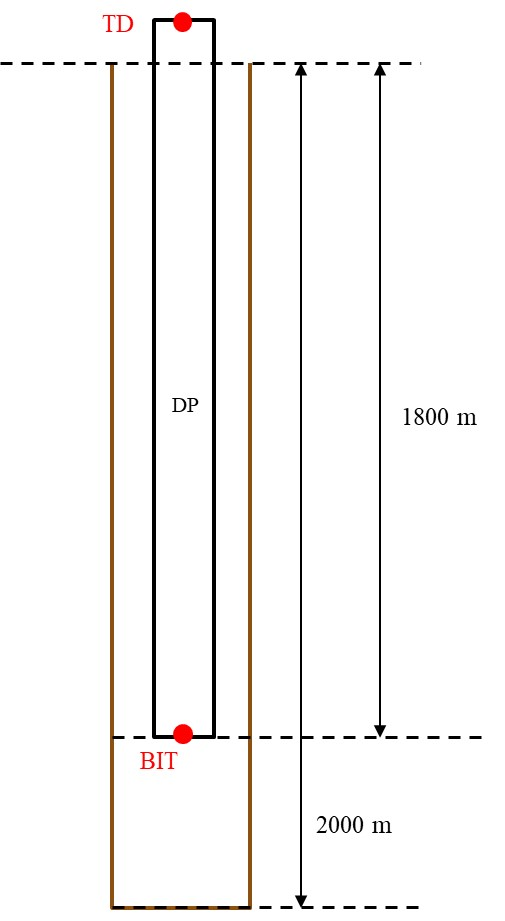
\includegraphics[width=1.5in]{VerticalWellConfig}
  \caption[Schematic of well and drill string for model comparison.]{Schematic of well and drill string for model comparison.}\label{figure_verticalwell}
\end{figure}

\begin{testcasetable}
$\rho$ & $490.6\;lb/ft^3$ & $7850\;kg/m^3$ & Drill pipe density \\                                                  
\hline
G & $1.67e^9\;lbf/ft^2$ & $7.99e^{10}\;Pa$  & Shear modulus \\                                                  
\hline
OD & 5.88 in & 0.15 m & drill pipe outer diameter\\                                                       
\hline
ID & 5.00 in & 0.127 m & drill pipe inner diameter  \\                                                      
\hline
MD & 6561 ft & 2000 m & measured depth\\                                                              
\hline
TVD & 6561 ft & 2000 m & total vertical depth\\
\hline
Bit depth & 5905 ft & 1800 m & - \\ 
\hline
\end{tabularx}
\caption[Well survey data for model comparison (vertical well)]{Well survey and drill string data for model comparison (vertical well without BHA components)}\label{table_verticalwell_input}
\end{testcasetable}
The test was conducted by assuming the top drive velocity to be increased from 0 RPM to 40 RPM at 1 second and maintained the velocity for rest of the time. The top drive velocity is shown in \figurename~\ref{figure_topdrive_VSP}

\begin{figure}[!hbt]
  \centering
  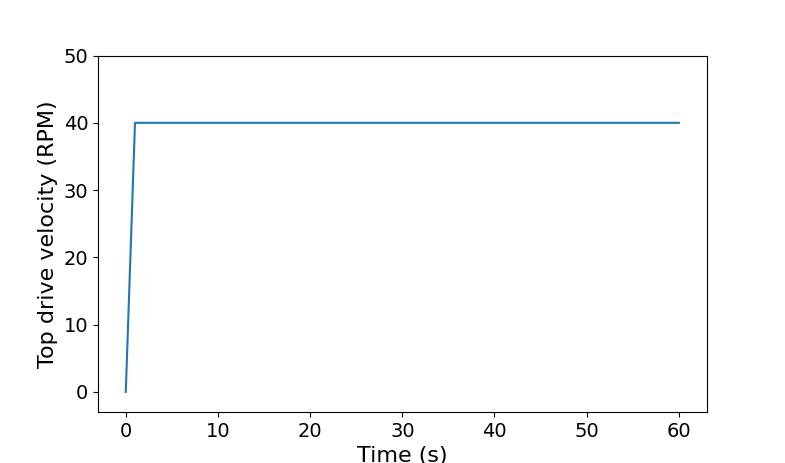
\includegraphics[width=3in]{TopdriveVSP}
  \caption[Top drive set velocity]{Top drive set velocity}\label{figure_topdrive_VSP}
\end{figure}

%Comparison between A-S model (both Matlab ver.\ and Python ver.\), and Exxon mobil model was conducted with given input in \tablename~\ref{table_verticalwell_input}. The modified code of PYTHON ver.\ with removed top drive was used for the comparison. First, for the simplicity, the viscous damping was assumed to be zero. Moreover, the coulomb friction is also zero since there is no contact between drill string and borehole (vertical well). Therefore the source term of the governing equation will be zero in equation \equationname~\ref{AS-motion} and the parameters that affect the model will be the density and shear modulus of drill pipe.
%
%The comparison between different models are shown in \figurename~\ref{figure_modelcomparison_vertical_torque}. As can be seen from the results all the model showed  oscillation of the top drive torque, however, significant difference were observed in A-S model PYTHON ver.\ while MATLAB ver.\, and exxon mobil model shwed maximum torque about 2000 lb-ft, torque of the PYTHON ver.\ reached 10,000 lb-ft. Also, the differences in the oscillation frequencies were observed. The frequency of oscillation were 0.32, 0.45, and 0.125 for MATLAB ver.\, and Exxon mobil model, and PYTHON ver.\, respectively. Although MATLAB ver.\ and Exxon mobil model showed similar response, the convergence time of this oscillation were significantly shorter in MATLAB ver.\ The comparison of the converging time between MATLAB ver.\ and PYTHON ver.\ is illustrated in \figurename~\ref{figure_modelcomparison_vertical_convergence}. The comparison of the model are summerized in Table....

%\begin{figure}[hbt!]
%  \centering
%  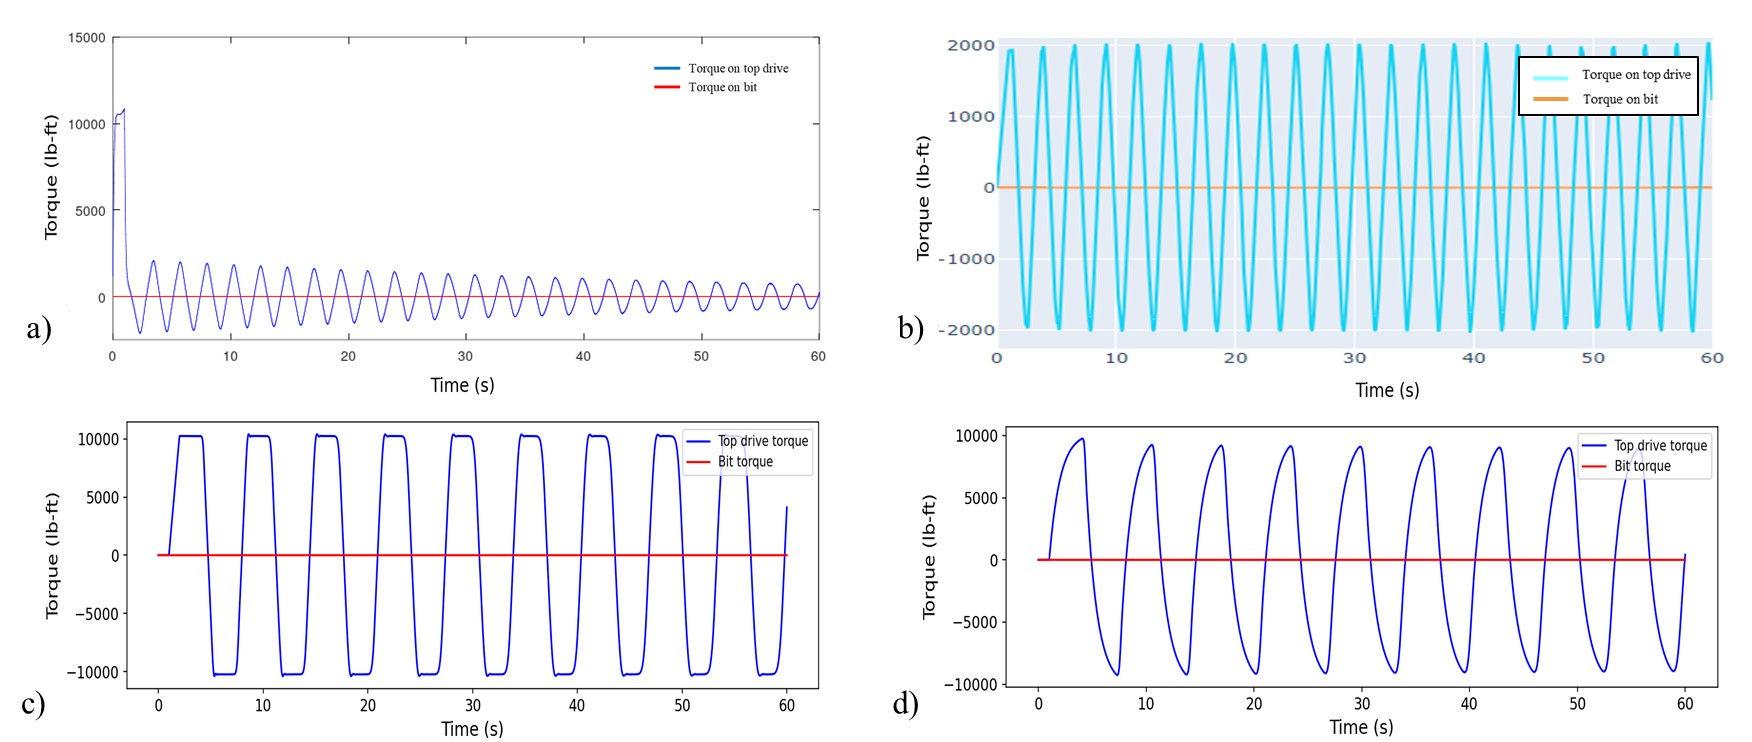
\includegraphics[width=6in]{modelcomparison_vertical_torque}
%  \caption[Comparison of torque of top drive and bit without viscous damping and BHA components in vertical well]{Comparison of torque of top drive and bit without viscous damping and BHA components in vertical well. the input parameteres for drill string is summarized in \tablename~\ref{table_verticalwell_input}. a): A-S model (MATLAB ver.\), b): Exxon mobil model, c) A-S model (PYTHON ver.\), and d): A-S model (PYTHON ver.\) with smooth increase of top drive velocity.}\label{figure_modelcomparison_vertical_torque}
%\end{figure}
%
%\begin{figure}
%  \centering
%  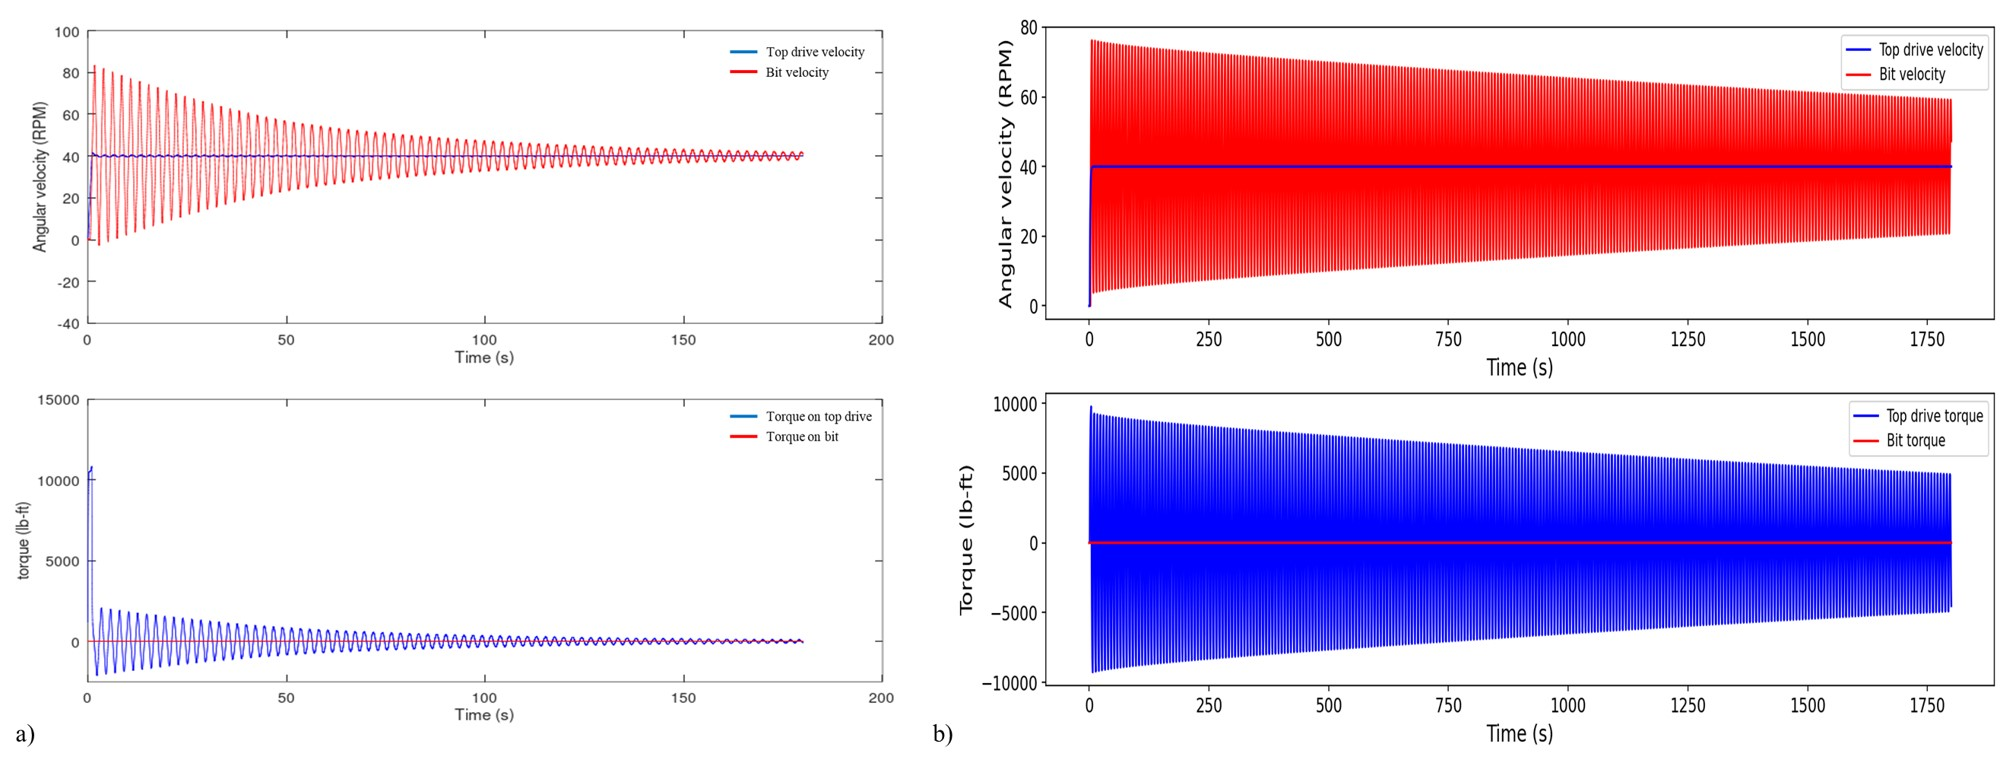
\includegraphics[width=6.5in]{modelcomparison_vertical_convergence}
%  \caption[Comparison of torsional vibration convergence time without viscous damping and BHA components in vertical well.]{Comparison of torsional vibration convergence time without viscous damping and BHA components in vertical well. a): A-S model MATLAB ver.\, b): A-S model PYTHON ver.}\label{figure_modelcomparison_vertical_convergence}
%\end{figure}
%
%%\begin{table}[!hbt]
%%\centering
%%\begin{tabular}{|c|c}|c|c|}
%%\hline
%% & Exxon mobil model & A-S model (MATLAB ver.\) & A-S model (PYTHON ver.\) \\                                                              
%%\hline
%%Drill string vibration convergence & - & $<$ 150s & $>$ 30min \\                                                  
%%\hline
%%Vibration frequency & 0.32 & 0.45  & 0.125 \\                                                  
%%\hline
%%Maximum torque on top drive (lb-ft) & 2000 in & 2000 & \\                                                       
%%\hline
%%\end{tabular}
%%\caption[Summary of model comparison without damping and BHA components in vertical well.]{Summary of model comparison without damping and BHA components in vertical well.}\label{table_modelcomparison_vertical_input}
%%\end{table}

\section{Test Case 2 - Inclined well, No BHA}
\subsection{Test Case 2a - Different Friction Factor values}

The models were tested with inclined well with simple configuration of drill string. The MD of the well is 4000 m with 60 deg inclination. The drill bit is off-bottom where located at 2500 m depth. The Schematic view of wellbore and drill string are depicted in \figurename~\ref{figure_wellconfig_inclined}. Also, the top drive velocity is increased to 40 RPM at 1 second which is same with test case 1 (\figurename\ref{figure_topdrive_VSP}). For test case 2, the viscous damping is neglected for the simplicity of the test. However, Coulomb friction is considered to investigate the stick-slip occurrence during drilling. The parameters for the test are summarized in \tablename~\ref{table_Inclinedwell_2a_input}.

\begin{figure}[!hbt]
  \centering
  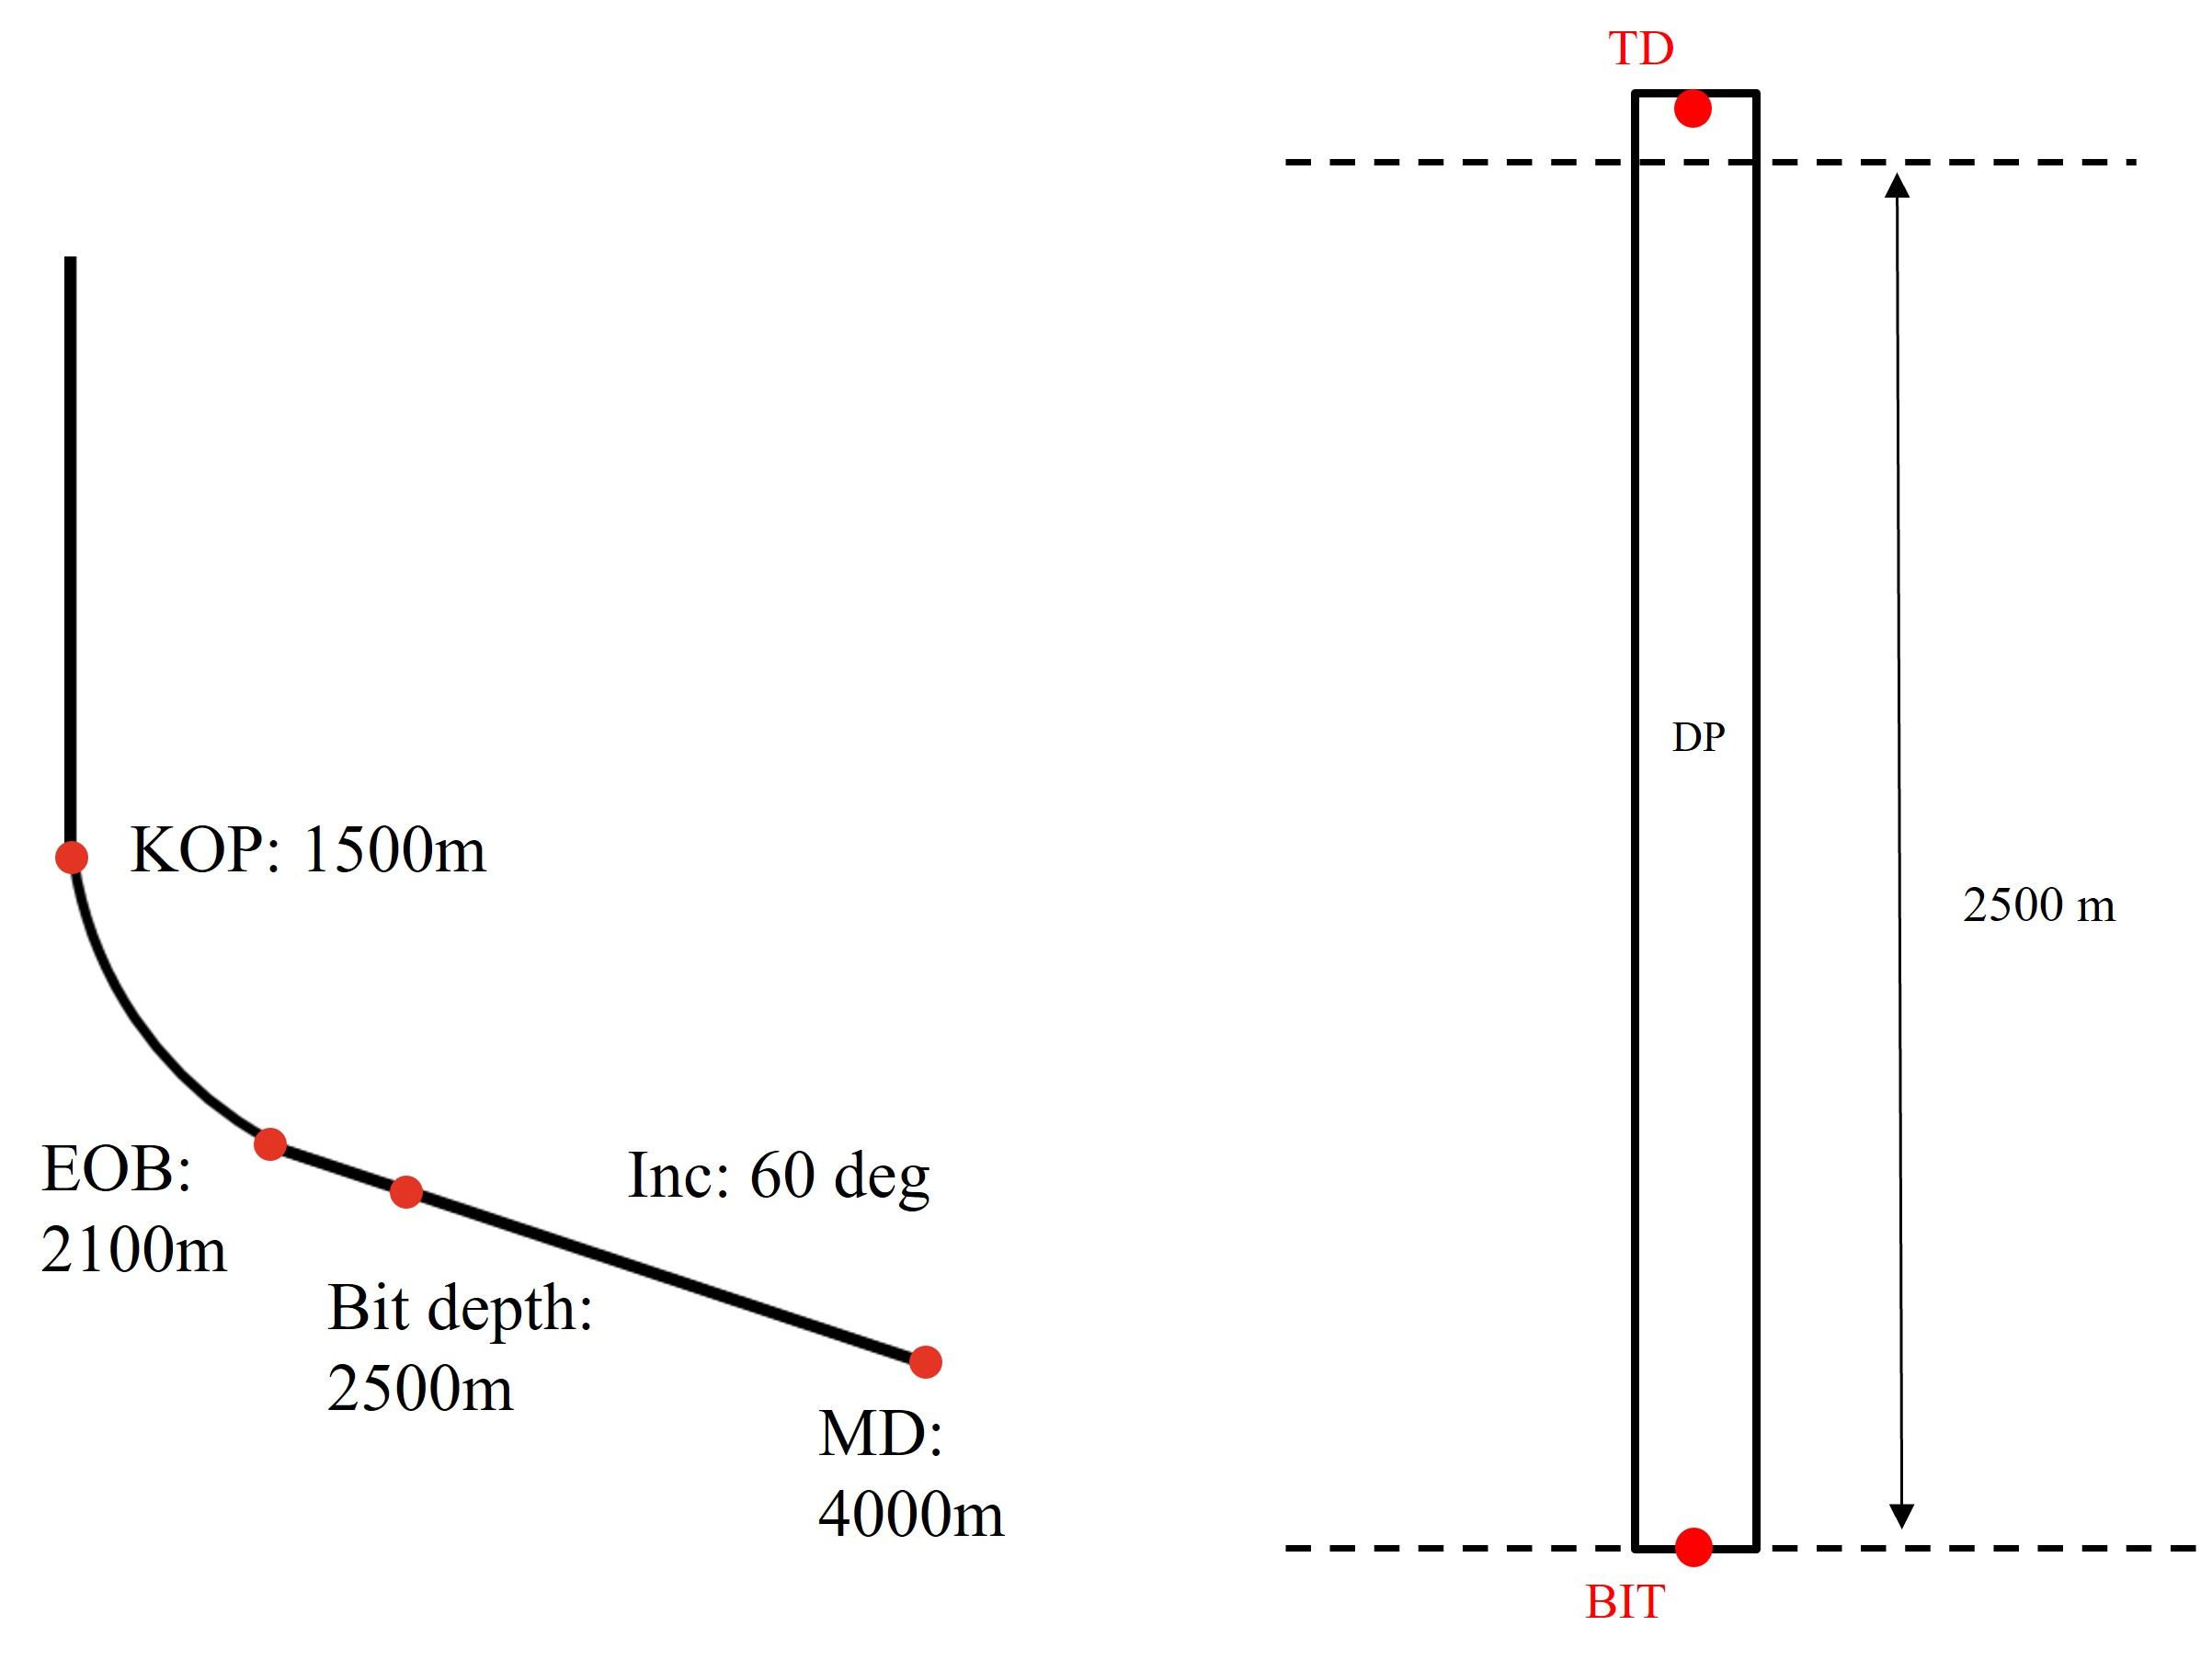
\includegraphics[width=4in]{InclinedWellConfig}
  \caption[Schematic view of test case 2.]{Schematic view of wellbore and drill string for test case 2.}\label{figure_wellconfig_inclined}
\end{figure}

\begin{testcasetable}
   $OD_{dp}$ & 5.88 in & 0.15 m & drill pipe outer diameter\\                                                       
   \hline
   $ID_{dp}$ & 5.00 in & 0.127 m & drill pipe inner diameter  \\                                                      
   \hline
   $\rho_{dp}$ & $490.6\;lb/ft^3$ & $7850\;kg/m^3$ & Drill pipe density \\                                                  
   \hline
   $G_{dp}$ & $1.27e^{9}\;lb/ft^2$ & $6.10e^{10}\;pa$ & drill pipe shear modulus\\                                                              
   \hline
   $\mu_{s}$ & 0.5 & 0.5 & Static friction factor\\
   \hline
   $\mu_{d}$ & 0.25 & 0.25 & Static friction factor\\
   \hline
   $w_c$ & 10 RPM & 10 RPM & Cut-off angular velocity\\
   \hline
   $\theta$ & $60^{\circ}$ & $60^{\circ}$ & Inclination\\
   \hline
   \end{tabularx}
\caption[Input parameters for test case 2a]{Input parameters for test case 2a.}\label{table_Inclinedwell_2a_input}
\end{testcasetable}


\subsection{Test case 2b - Same Friction Factor values}

The models were tested with the exact same configuration from the previous subsection, except with same values of Static and Dynamic FF (Friction Factor) values. The following \tablename~\ref{table_Inclinedwell_2b_input} summarizes the input parameters. 

\begin{testcasetable}
  $OD_{dp}$ & 5.88 in & 0.15 m & drill pipe outer diameter\\                                                       
  \hline
  $ID_{dp}$ & 5.00 in & 0.127 m & drill pipe inner diameter  \\                                                      
  \hline
  $\rho_{dp}$ & $490.6\;lb/ft^3$ & $7850\;kg/m^3$ & Drill pipe density \\                                                  
  \hline
  $G_{dp}$ & $1.27e^{9}\;lb/ft^2$ & $6.10e^{10}\;pa$ & drill pipe shear modulus\\                                                              
  \hline
  $\mu_{s}$ & 0.5 & 0.5 & Static friction factor\\
  \hline
  $\mu_{d}$ & 0.5 & 0.5 & Static friction factor\\
  \hline
  $w_c$ & 10 RPM & 10 RPM & Cut-off angular velocity\\
  \hline
  $\theta$ & $60^{\circ}$ & $60^{\circ}$ & Inclination\\
  \hline
  \end{tabularx}
\caption[Input parameters for test case 2b]{Input parameters for test case 2b.}\label{table_Inclinedwell_2b_input}
\end{testcasetable}

%The results from A-S models are shown in \figurename~\ref{figure_testcase2_ASmodel}. Both model captured the stick-slip event during of-bottom drill string rotation. However, similar to test case 1 (have to rename it later: vertical well test), the top drive torque amplitude and the frequency of the oscillation showed significant differences.
% 
%\begin{figure}[!hbt]
%  \centering
%  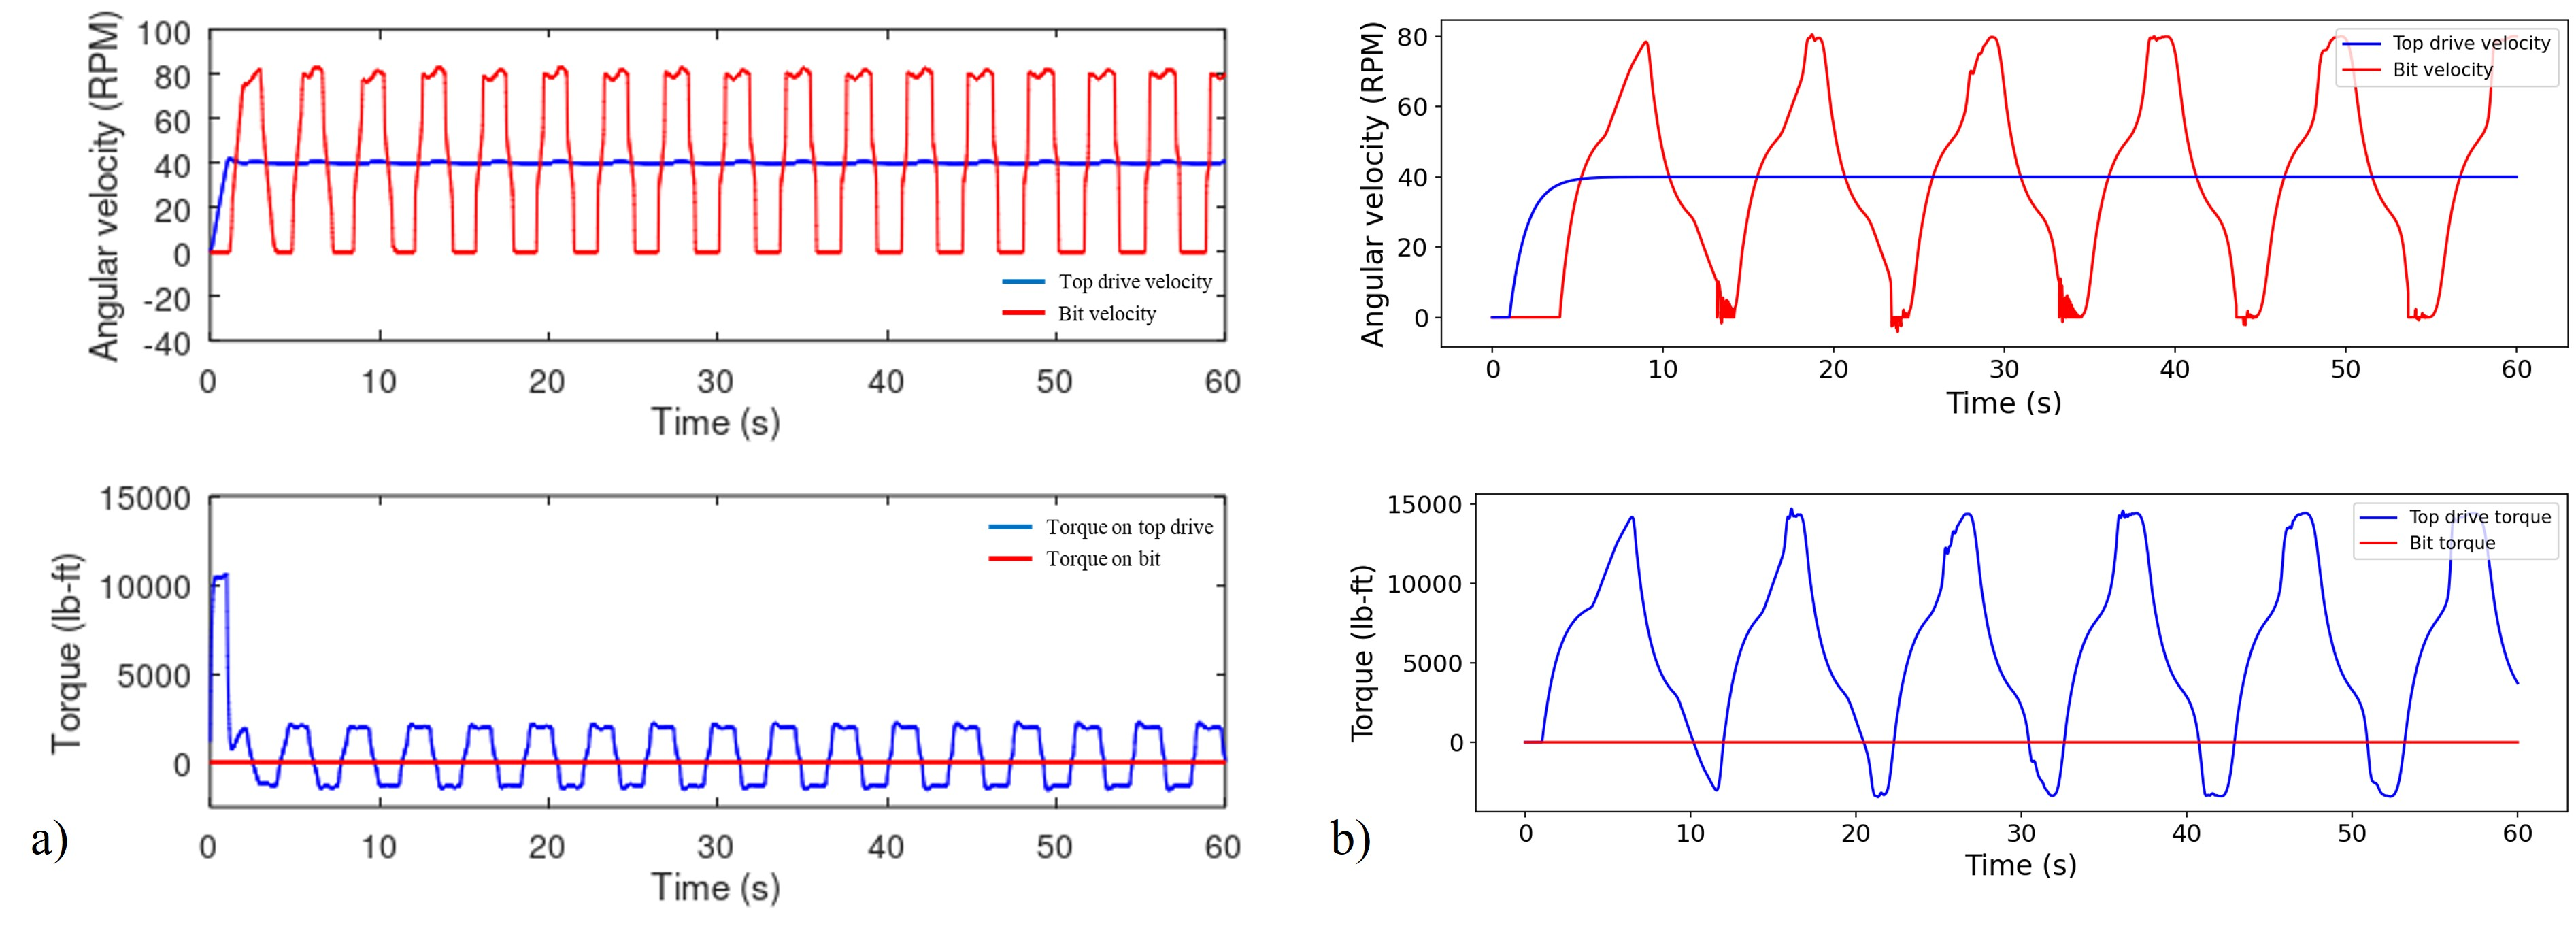
\includegraphics[width=6.5in]{Testcase2_ASmodel}
%  \caption[Result from A-S model. (test case 2)]{Simulation results of A-S model for test case 2, a): MATLAB ver, and b): PYTHON ver.\ Stick-slip was observed from the model.}\label{figure_testcase2_ASmodel}
%\end{figure}
%
%
%A-S model
%\begin{numberedlist}
%	\item Difference in torque amplitude
%	\item Difference in oscillation frequencies
%	\item Bit model - constant torque
%	\item Comparison using color map?
%\end{numberedlist}

\section{Test Case 3 - Vertical Well with BHA}

In this specific scenario, an additional configuration of the drill string included a Bottom Hole Assembly (BHA). The BHA introduced extra components, resulting in an increase in both the weight and size of the drill string. However, the well survey data for the vertical well remained the same, except for the incorporation of the BHA. The well design, depicted in \figurename~\ref{Vert_well_conf_BHA}, remained unchanged, as well as, the parameters for the top drive. For the sake of simplicity, the influence of viscous damping was disregarded. The specific input parameters can be found in the \tablename~\ref{Input Parameters TC3}.

\begin{figure}
  \centering
  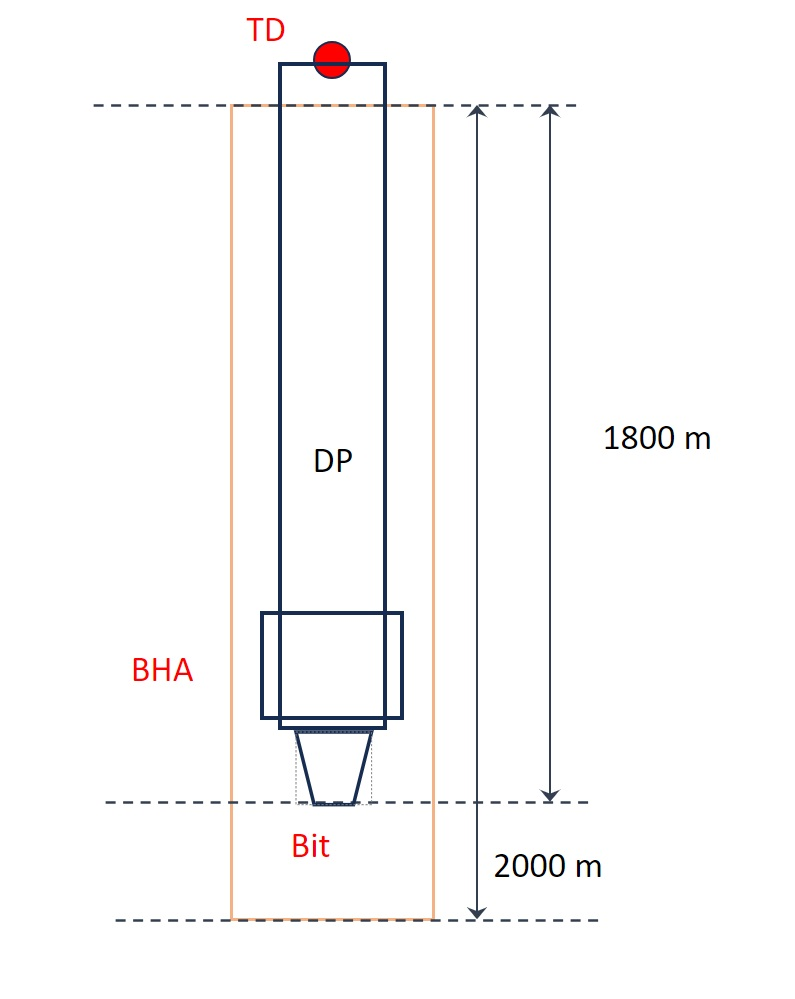
\includegraphics[width=2in]{VerticalWellConfigBHA}
  \caption{Schematic of well and drill string for model comparison}\label{Vert_well_conf_BHA}
\end{figure}


\begin{testcasetable}
    $OD_{HWDP}$ & 4.50 in & 0.1143 m & Heavy weight drill pipe outer diameter \\
    \hline
    $ID_{HWDP}$ & 2.50 in & 0.0635 m & Heavy weight drill pipe inner diameter \\
    \hline
    $OD_{DC}$ & 6.00 in & 0.1524 m & Drill collars outer diameter \\
    \hline
    $ID_{DC}$ & 2.00 in & 0.0508 m & Drill collars inner diameter \\
    \hline
    $L_{HWDP}$ & 60 ft & 18.30 m & Length of heavy weight drill pipe \\
    \hline
    $L_{DC}$ & 270 ft & 82.30 m & Length of drill collars \\
    \hline
    $\rho_{dp}$ & 490.6 $lb/ft^{3}$ & 7850 $kg/m^{3}$ & Drill pipe density \\
    \hline
    $G_{dp}$ & $1.67e^9\;lbf/ft^2$ & $7.99e^{10}\;Pa$ & Drill pipe shear modulus \\
    \hline
    \end{tabularx}
  \caption{Input parameters of BHA for test case 3}\label{Input Parameters TC3}
\end{testcasetable} 

\section{Test Case 4 - Inclined Well with BHA}
\subsection{Test Case 4a - Different Friction Factor values}

The models were tested with the same input parameters from test case 2, with additional configuration of the drill string including a Bottom Hole Assembly (BHA). Well survey data for the inclined well remained same, except for the incorporation of the BHA. The well design, depicted in \figurename~\ref{figure_wellconfig_inclined_BHA}, remained unchanged, as well as, the parameters for the top drive. As stated previously in test case 2 the influence of viscous damping was disregarded. The input parameters can be found in the  \tablename~\ref{table_Inclinedwell_4a_input}.

\begin{figure}[!hbt]
  \centering
  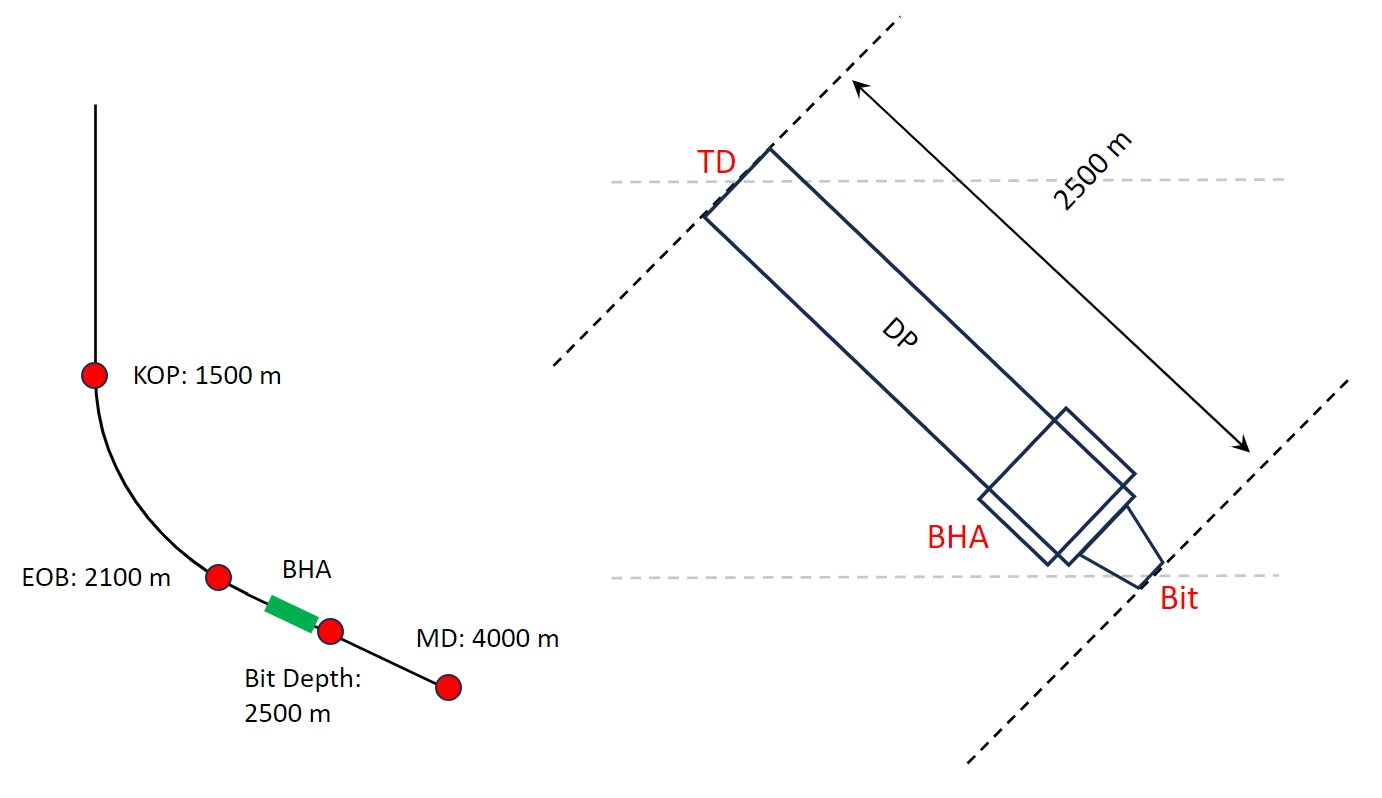
\includegraphics[width=4in]{InclinedWellConfigBHA}
  \caption[Schematic view of test case 4.]{Schematic view of wellbore and drill string for test case 4.}\label{figure_wellconfig_inclined_BHA}
\end{figure}

\begin{testcasetable}
   $OD_{HWDP}$ & 4.50 in & 0.1143 m & Heavy weight drill pipe outer diameter \\   
   \hline
   $ID_{HWDP}$ & 2.50 in & 0.0635 m & Heavy weight drill pipe inner diameter \\
   \hline
   $OD_{DC}$ & 6.00 in & 0.1524 m & Drill collars outer diameter \\
   \hline
   $ID_{DC}$ & 2.00 in & 0.0508 m & Drill collars inner diameter \\                                                    
   \hline
   $L_{HWDP}$ & 60 ft & 18.30 m & Length of heavy weight drill pipe \\
   \hline
   $L_{DC}$ & 270 ft & 82.30 m & Length of drill collars \\
   \hline
   $\rho_{dp}$ & $490.6\;lb/ft^3$ & $7850\;kg/m^3$ & Drill pipe density \\                                                  
   \hline
   $G_{dp}$ & $1.27e^{9}\;lb/ft^2$ & $6.10e^{10}\;pa$ & drill pipe shear modulus\\                                                              
   \hline
   $\mu_{s}$ & 0.5 & 0.5 & Static friction factor\\
   \hline
   $\mu_{d}$ & 0.25 & 0.25 & Static friction factor\\
   \hline
   $w_c$ & 10 RPM & 10 RPM & Cut-off angular velocity\\
   \hline
   $\theta$ & $60^{\circ}$ & $60^{\circ}$ & Inclination\\
   \hline
   \end{tabularx}
   \caption[Input parameters for test case 4a]{Input parameters for test case 4a.}\label{table_Inclinedwell_4a_input}
\end{testcasetable}

\subsection{Test Case 4b - Same Friction Factor values}

Lastly, the models were tested with the exact same configuration from the previous subsection, except with same values of Static and Dynamic FF (Friction Factor) values. The following \tablename~\ref{table_Inclinedwell_4b_input} summarizes the input parameters. 

\begin{testcasetable}
   $OD_{HWDP}$ & 4.50 in & 0.1143 m & Heavy weight drill pipe outer diameter \\
   \hline
   $ID_{HWDP}$ & 2.50 in & 0.0635 m & Heavy weight drill pipe inner diameter \\
   \hline
   $OD_{DC}$ & 6.00 in & 0.1524 m & Drill collars outer diameter \\
   \hline
   $ID_{DC}$ & 2.00 in & 0.0508 m & Drill collars inner diameter \\                                                    
   \hline
   $L_{HWDP}$ & 60 ft & 18.30 m & Length of heavy weight drill pipe \\
   \hline
   $L_{DC}$ & 270 ft & 82.30 m & Length of drill collars \\
   \hline
   $\rho_{dp}$ & $490.6\;lb/ft^3$ & $7850\;kg/m^3$ & Drill pipe density \\                                                  
   \hline
   $G_{dp}$ & $1.27e^{9}\;lb/ft^2$ & $6.10e^{10}\;pa$ & drill pipe shear modulus\\                                                              
   \hline
   $\mu_{s}$ & 0.5 & 0.5 & Static friction factor\\
   \hline
   $\mu_{d}$ & 0.5 & 0.5 & Static friction factor\\
   \hline
   $w_c$ & 10 RPM & 10 RPM & Cut-off angular velocity\\
   \hline
   $\theta$ & $60^{\circ}$ & $60^{\circ}$ & Inclination\\
   \hline
   \end{tabularx}
\caption[Input parameters for test case 4b.]{Input parameters for test case 4b.}\label{table_Inclinedwell_4b_input}
\end{testcasetable}
